%%%%%%%%%%%%%%%%%%%%%%%%%%%%%%%%%%%%%%%%%
% Professional Mathematical Presentation Template
% 
% This template uses the beamer class with the Madrid theme
% and a custom color scheme for a clean, professional look
% that works well with mathematical content.
%%%%%%%%%%%%%%%%%%%%%%%%%%%%%%%%%

\documentclass[aspectratio=169]{beamer} % 16:9 aspect ratio (modern)

% Theme settings
\usetheme{Madrid}
\usecolortheme{default}

\definecolor{primcolor}{RGB}{25,50,100} % Dark blue
\setbeamercolor{structure}{fg=primcolor}
\setbeamercolor{frametitle}{bg=primcolor!15, fg=primcolor}
\setbeamercolor{title}{fg=white} % White title text for contrast
\setbeamercolor{subtitle}{fg=white} % White subtitle text
\setbeamercolor{author}{fg=primcolor} % White author text
\setbeamercolor{date}{fg=primcolor} % White date text
\setbeamercolor{institute}{fg=primcolor} % White institute text

% Font settings
\usefonttheme{professionalfonts}
\usefonttheme{serif}

% Package imports
\usepackage{amsmath, amsfonts, amssymb, amsthm} % Math packages
\usepackage{mathtools} % Enhanced math tools
\usepackage{bm} % Bold math symbols
\usepackage{graphicx} % For images
\usepackage{booktabs} % Professional tables
\usepackage{tikz} % For diagrams
\usetikzlibrary{arrows, arrows.meta, positioning, matrix, decorations.pathreplacing, shapes.geometric, calc, patterns, shapes, mindmap}

% Use beamer's theorem styles
\setbeamertemplate{theorem}[ams style]
\setbeamertemplate{theorems}[numbered]

% Remove navigation symbols
\setbeamertemplate{navigation symbols}{}

% Custom footer
\setbeamertemplate{footline}{
  \leavevmode%
  \hbox{%
  \begin{beamercolorbox}[wd=.333333\paperwidth,ht=2.25ex,dp=1ex,center]{author in head/foot}%
    \usebeamerfont{author in head/foot}\insertshortauthor
  \end{beamercolorbox}%
  \begin{beamercolorbox}[wd=.333333\paperwidth,ht=2.25ex,dp=1ex,center]{title in head/foot}%
    \usebeamerfont{title in head/foot}\insertshorttitle
  \end{beamercolorbox}%
  \begin{beamercolorbox}[wd=.333333\paperwidth,ht=2.25ex,dp=1ex,right]{date in head/foot}%
    \usebeamerfont{date in head/foot}\insertshortdate{}\hspace*{2em}
    \insertframenumber{} / \inserttotalframenumber\hspace*{2ex} 
  \end{beamercolorbox}}%
  \vskip0pt%
}

% Title information
\title[DRL]{Deep Reinforcement Learning can promote sustainable human behaviour in common-pool resource problems}
\subtitle{Koster et al. 2025}
\author[Longye]{Longye Tian \\ \texttt{longye.tian@anu.edu.au}}
\institute[ANU]{Australian National University\\ School of Economics}
\date{March 27th, 2025}
\DeclareFontFamily{U}{mathx}{\hyphenchar\font45}
\DeclareFontShape{U}{mathx}{m}{n}{
      <5> <6> <7> <8> <9> <10>
      <10.95> <12> <14.4> <17.28> <20.74> <24.88>
      mathx10
      }{}
\DeclareSymbolFont{mathx}{U}{mathx}{m}{n}
\DeclareMathSymbol{\bigtimes}{1}{mathx}{"91}

\begin{document}

% Title frame
\begin{frame}
  \titlepage
\end{frame}

% Outline frame
\begin{frame}{Outline}
  \begin{center}
  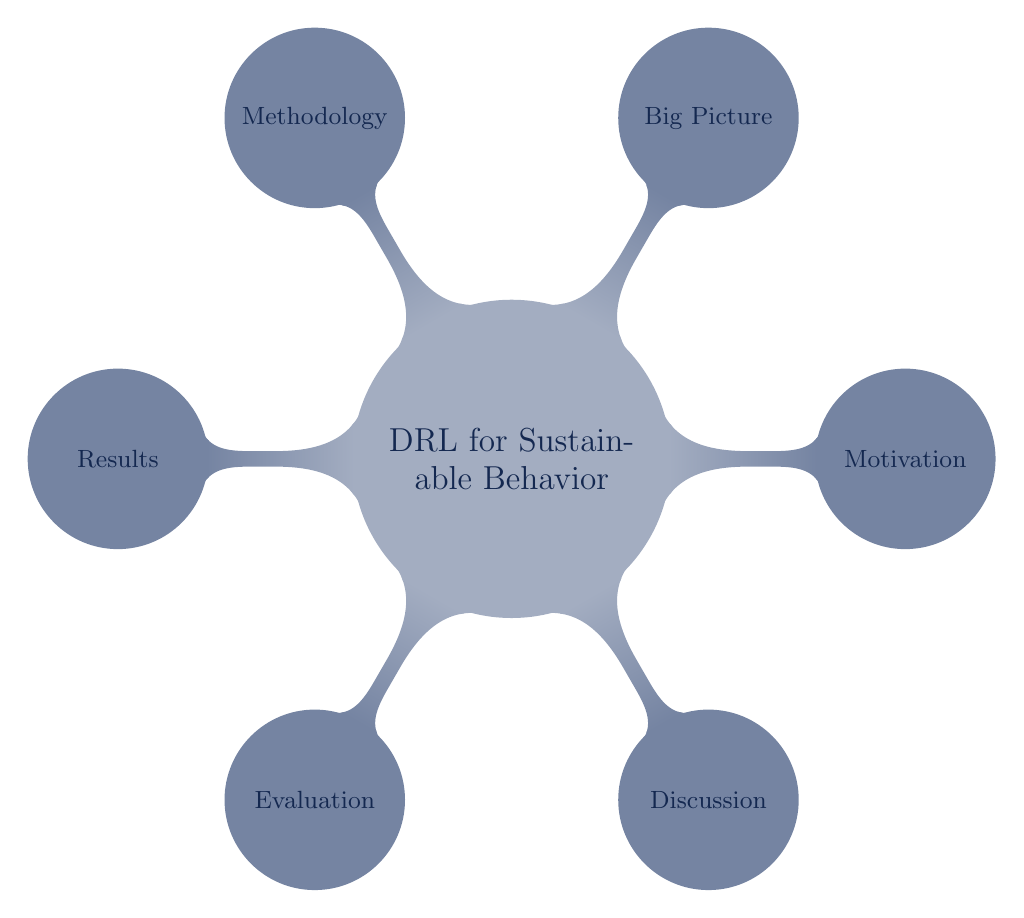
\begin{tikzpicture}[mindmap, concept color=primcolor!40, text=primcolor!80!black]
    \node[concept] {DRL for Sustainable Behavior}
      child[concept color=primcolor!60, grow=0] { node[concept] {Motivation} }
      child[concept color=primcolor!60, grow=60] { node[concept] {Big Picture} }
      child[concept color=primcolor!60, grow=120] { node[concept] {Methodology} }
      child[concept color=primcolor!60, grow=180] { node[concept] {Results} }
      child[concept color=primcolor!60, grow=240] { node[concept] {Evaluation} }
      child[concept color=primcolor!60, grow=300] { node[concept] {Discussion} };
  \end{tikzpicture}
  \end{center}
\end{frame}

\section{Motivation}
\begin{frame}{Motivation}
\begin{center}
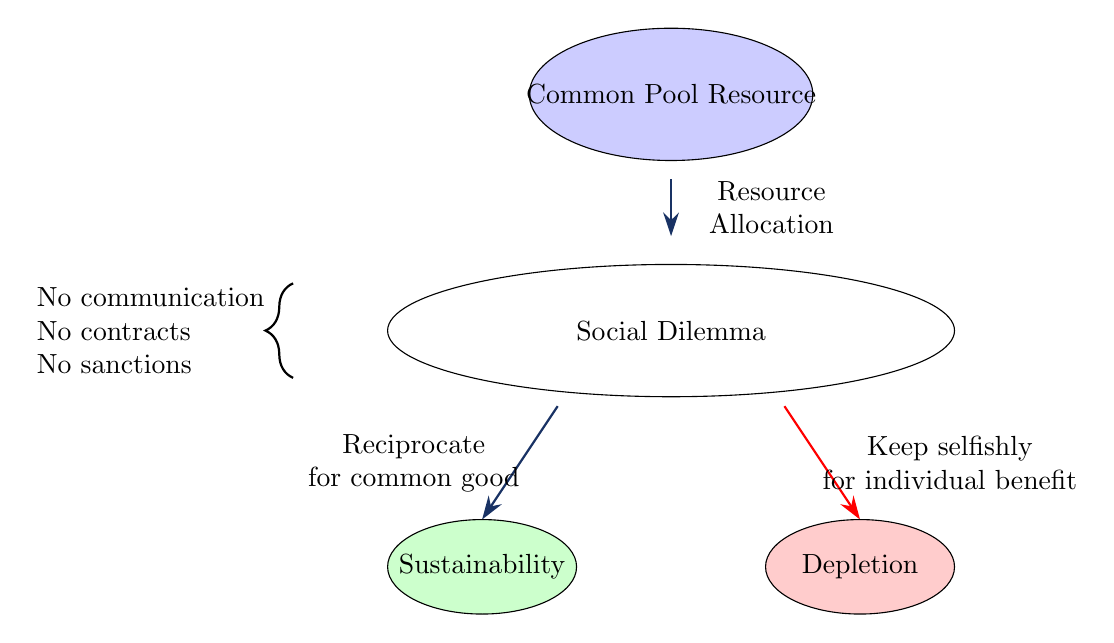
\begin{tikzpicture}[scale=1.2]
    % Common pool resource
    \draw[fill=blue!20] (0,3.5) ellipse (1.5cm and 0.7cm);
    \node at (0,3.5) {Common Pool Resource};
    
    % Downward arrow
    \draw[-{Stealth[length=3mm, width=2mm]}, thick, primcolor] (0,2.6) -- (0,2);
    \node[align=center, right] at (0.3,2.3) {Resource\\Allocation};
    
    % Social dilemma
    \draw (0,1) ellipse (3cm and 0.7cm);
    \node at (0,1) {Social Dilemma};
    
    % Individual choices
    \draw[-{Stealth[length=3mm, width=2mm]}, thick, primcolor] (-1.2,0.2) -- (-2,-1);
    \node[align=center, left] at (-1.5,-0.4) {Reciprocate\\for common good};
    
    \draw[-{Stealth[length=3mm, width=2mm]}, thick, red] (1.2,0.2) -- (2,-1);
    \node[align=center, right] at (1.5,-0.4) {Keep selfishly\\for individual benefit};
    
    % Outcomes
    \draw[fill=green!20] (-2,-1.5) ellipse (1cm and 0.5cm);
    \node at (-2,-1.5) {Sustainability};
    
    \draw[fill=red!20] (2,-1.5) ellipse (1cm and 0.5cm);
    \node at (2,-1.5) {Depletion};
    
    % Challenge: no communication
    \draw[decorate, decoration={brace,amplitude=10pt}, thick] (-4,0.5) -- (-4,1.5);
    \node[align=left, anchor=east] at (-4.2,1) {No communication\\No contracts\\No sanctions};
\end{tikzpicture}
\end{center}

\vspace{-0.3cm}
\begin{center}
\textbf{Goal:} Find resource allocation rules that encourage sustainable behavior
\end{center}
\end{frame}

\begin{frame}{The Problem in Context}
\begin{center}
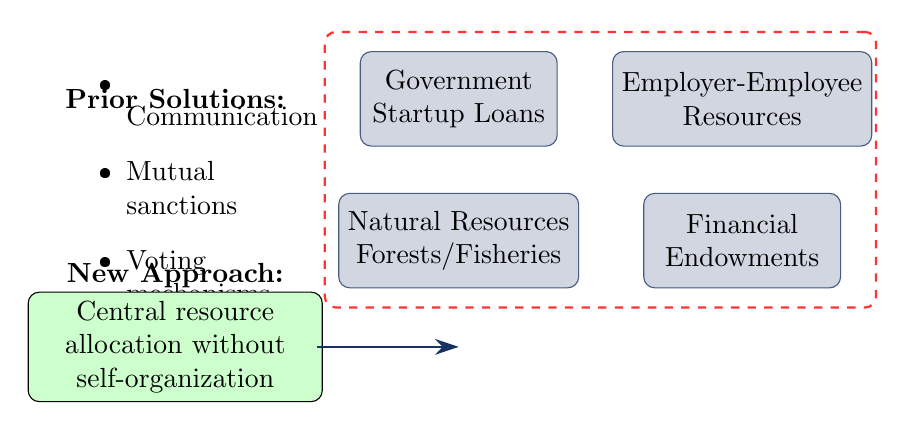
\begin{tikzpicture}[scale=0.9]
    % Real-world examples
    \node[draw=primcolor!80, fill=primcolor!20, rounded corners, align=center, minimum width=2.5cm, minimum height=1.2cm] (gov) at (0,2) {Government\\Startup Loans};
    
    \node[draw=primcolor!80, fill=primcolor!20, rounded corners, align=center, minimum width=2.5cm, minimum height=1.2cm] (emp) at (4,2) {Employer-Employee\\Resources};

    \node[draw=primcolor!80, fill=primcolor!20, rounded corners, align=center, minimum width=2.5cm, minimum height=1.2cm] (res) at (0,0) {Natural Resources\\Forests/Fisheries};
    
    \node[draw=primcolor!80, fill=primcolor!20, rounded corners, align=center, minimum width=2.5cm, minimum height=1.2cm] (fin) at (4,0) {Financial\\Endowments};
    
    % Common characteristics
    \node[draw=red!80, thick, dashed, rounded corners, align=center, minimum width=7cm, minimum height=3.5cm] at (2,1) {};
    
    % Prior solutions
    \node[align=left] at (-4,2) {\textbf{Prior Solutions:}};
    \node[align=left, text width=3cm] at (-4,1) {
        \begin{itemize}
            \item Communication
            \item Mutual sanctions
            \item Voting mechanisms
        \end{itemize}
    };
    
    % New approach
    \node[align=left] at (-4,-0.5) {\textbf{New Approach:}};
    \node[align=center, text width=3.5cm, fill=green!20, rounded corners, draw] at (-4,-1.5) {Central resource allocation without self-organization};
    
    % Arrow
    \draw[-{Stealth[length=3mm, width=2mm]}, thick, primcolor] (-2,-1.5) -- (0,-1.5);
\end{tikzpicture}
\end{center}
\end{frame}

\section{Big Picture}

\begin{frame}{Main Idea}
\begin{center}
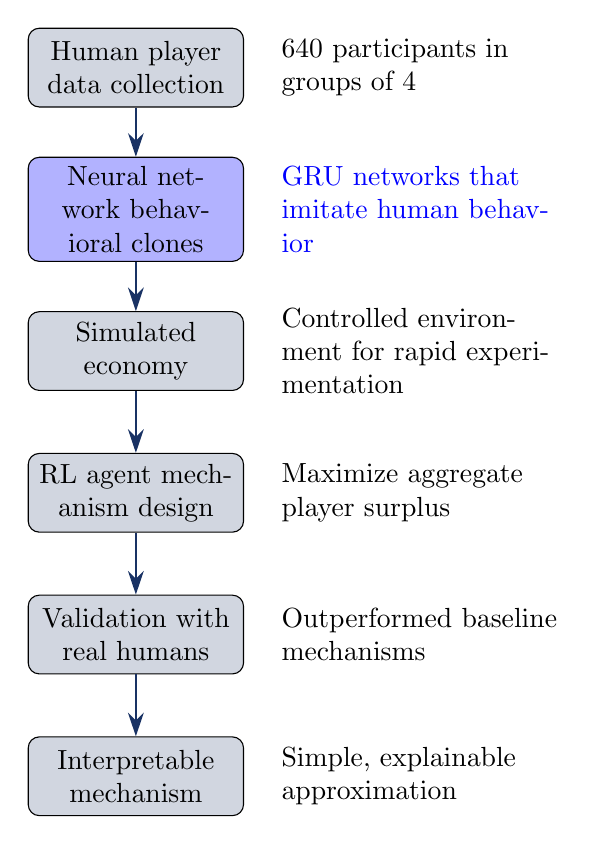
\begin{tikzpicture}[
    block/.style={draw, rounded corners, fill=primcolor!20, text width=2.5cm, minimum height=1cm, align=center},
    arrow/.style={-{Stealth[length=3mm, width=2mm]}, thick, primcolor},
    scale=0.9
]
    % Blocks in sequence
    \node[block] (data) at (0,0) {Human player data collection};
    \node[block, fill=blue!30] (clones) at (0,-2) {Neural network behavioral clones};
    \node[block] (sim) at (0,-4) {Simulated economy};
    \node[block] (rl) at (0,-6) {RL agent mechanism design};
    \node[block] (test) at (0,-8) {Validation with real humans};
    \node[block] (interpret) at (0,-10) {Interpretable mechanism};
    
    % Connect blocks with arrows
    \draw[arrow] (data) -- (clones);
    \draw[arrow] (clones) -- (sim);
    \draw[arrow] (sim) -- (rl);
    \draw[arrow] (rl) -- (test);
    \draw[arrow] (test) -- (interpret);
    
    % Annotations
    \node[text width=3.5cm, align=left] at (4,0) {640 participants in groups of 4};
    \node[text width=3.5cm, align=left, text=blue] at (4,-2) {GRU networks that imitate human behavior};
    \node[text width=3.5cm, align=left] at (4,-4) {Controlled environment for rapid experimentation};
    \node[text width=3.5cm, align=left] at (4,-6) {Maximize aggregate player surplus};
    \node[text width=3.5cm, align=left] at (4,-8) {Outperformed baseline mechanisms};
    \node[text width=3.5cm, align=left] at (4,-10) {Simple, explainable approximation};
\end{tikzpicture}
\end{center}
\end{frame}

\begin{frame}{The Game Structure}
\begin{center}
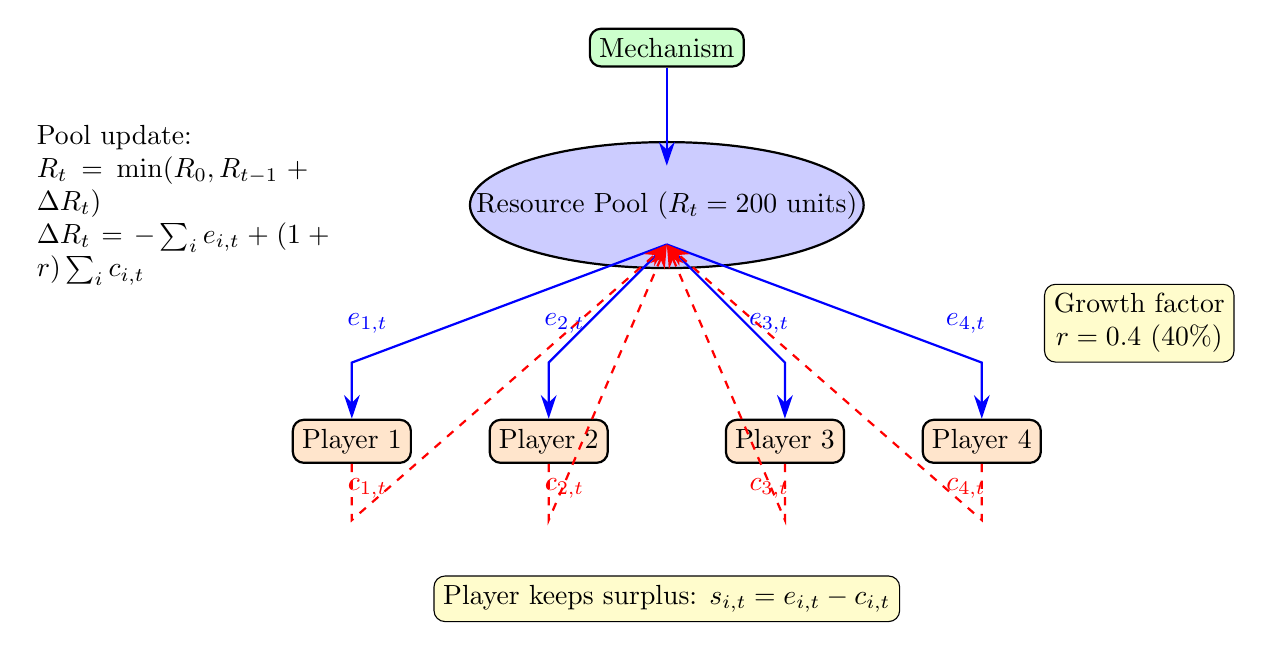
\begin{tikzpicture}[scale=1.0]
    % Pool
    \draw [fill=blue!20, thick] (0,3) ellipse (2.5cm and 0.8cm);
    \node at (0,3) {Resource Pool ($R_t = 200$ units)};
    
    % Mechanism
    \node[draw, thick, fill=green!20, rounded corners, align=center] (mech) at (0,5) {Mechanism};
    
    % Players
    \node[draw, thick, fill=orange!20, rounded corners] (p1) at (-4,0) {Player 1};
    \node[draw, thick, fill=orange!20, rounded corners] (p2) at (-1.5,0) {Player 2};
    \node[draw, thick, fill=orange!20, rounded corners] (p3) at (1.5,0) {Player 3};
    \node[draw, thick, fill=orange!20, rounded corners] (p4) at (4,0) {Player 4};
    
    % Arrows down - allocation
    \draw[-{Stealth[length=3mm, width=2mm]}, thick, blue] (mech) -- (0,4) -- (0,3.5);
    \draw[-{Stealth[length=3mm, width=2mm]}, thick, blue] (0,2.5) -- (-4,1) -- (p1);
    \draw[-{Stealth[length=3mm, width=2mm]}, thick, blue] (0,2.5) -- (-1.5,1) -- (p2);
    \draw[-{Stealth[length=3mm, width=2mm]}, thick, blue] (0,2.5) -- (1.5,1) -- (p3);
    \draw[-{Stealth[length=3mm, width=2mm]}, thick, blue] (0,2.5) -- (4,1) -- (p4);
    
    % Labels for allocation
    \node[blue] at (-3.8,1.5) {$e_{1,t}$};
    \node[blue] at (-1.3,1.5) {$e_{2,t}$};
    \node[blue] at (1.3,1.5) {$e_{3,t}$};
    \node[blue] at (3.8,1.5) {$e_{4,t}$};
    
    % Arrows up - reciprocation
    \draw[-{Stealth[length=3mm, width=2mm]}, thick, red, dashed] (p1) -- (-4,-1) -- (0,2.5);
    \draw[-{Stealth[length=3mm, width=2mm]}, thick, red, dashed] (p2) -- (-1.5,-1) -- (0,2.5);
    \draw[-{Stealth[length=3mm, width=2mm]}, thick, red, dashed] (p3) -- (1.5,-1) -- (0,2.5);
    \draw[-{Stealth[length=3mm, width=2mm]}, thick, red, dashed] (p4) -- (4,-1) -- (0,2.5);
    
    % Labels for reciprocation
    \node[red] at (-3.8,-0.6) {$c_{1,t}$};
    \node[red] at (-1.3,-0.6) {$c_{2,t}$};
    \node[red] at (1.3,-0.6) {$c_{3,t}$};
    \node[red] at (3.8,-0.6) {$c_{4,t}$};
    
    % Growth indicator
    \node[align=center, fill=yellow!20, rounded corners, draw] at (6,1.5) {Growth factor\\$r = 0.4$ (40\%)};
    
    % Updates
    \node[align=left, text width=4cm] at (-6,3) {Pool update:\\$R_t = \min(R_0, R_{t-1} + \Delta R_t)$\\$\Delta R_t = -\sum_i e_{i,t} + (1+r)\sum_i c_{i,t}$};
    
    % Player surplus
    \node[align=center, fill=yellow!20, rounded corners, draw] at (0,-2) {Player keeps surplus: $s_{i,t} = e_{i,t} - c_{i,t}$};
\end{tikzpicture}
\end{center}
\end{frame}

\section{Methodology}

\begin{frame}{Research Pipeline}
\begin{center}
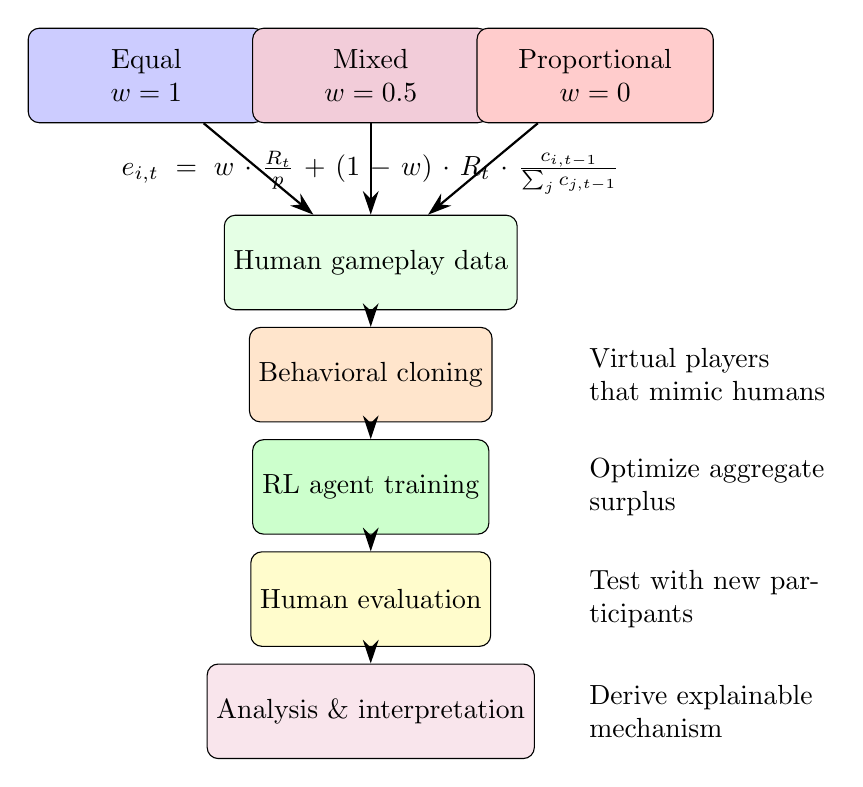
\begin{tikzpicture}[scale=0.95, 
    mech/.style={draw, rounded corners, minimum width=3cm, minimum height=1.2cm, align=center},
    arrow/.style={-{Stealth[length=3mm, width=2mm]}, thick}
]
    % Baseline mechanisms
    \node[mech, fill=blue!20] (equal) at (-3,2) {Equal\\$w = 1$};
    \node[mech, fill=purple!20] (mixed) at (0,2) {Mixed\\$w = 0.5$};
    \node[mech, fill=red!20] (prop) at (3,2) {Proportional\\$w = 0$};
    
    % Mixture formula
    \node[text width=8cm, align=center] at (0,0.7) {$e_{i,t} = w \cdot \frac{R_t}{p} + (1-w) \cdot R_t \cdot \frac{c_{i,t-1}}{\sum_j c_{j,t-1}}$};
    
    % Data collection
    \node[mech, fill=green!10] (data) at (0,-0.5) {Human gameplay data};
    
    % Behavioral cloning
    \node[mech, fill=orange!20] (clone) at (0,-2) {Behavioral cloning};
    
    % RL agent
    \node[mech, fill=green!20] (rl) at (0,-3.5) {RL agent training};
    
    % Evaluation
    \node[mech, fill=yellow!20] (eval) at (0,-5) {Human evaluation};
    
    % Analysis
    \node[mech, fill=purple!10] (analyze) at (0,-6.5) {Analysis \& interpretation};
    
    % Connect
    \draw[arrow] (equal) -- (data);
    \draw[arrow] (mixed) -- (data);
    \draw[arrow] (prop) -- (data);
    \draw[arrow] (data) -- (clone);
    \draw[arrow] (clone) -- (rl);
    \draw[arrow] (rl) -- (eval);
    \draw[arrow] (eval) -- (analyze);
    
    % Annotations
    \node[text width=3cm, align=left] at (4.5,-2) {Virtual players that mimic humans};
    \node[text width=3cm, align=left] at (4.5,-3.5) {Optimize aggregate surplus};
    \node[text width=3cm, align=left] at (4.5,-5) {Test with new participants};
    \node[text width=3cm, align=left] at (4.5,-6.5) {Derive explainable mechanism};
\end{tikzpicture}
\end{center}
\end{frame}

\begin{frame}{Behavioral Cloning}
\begin{center}
\begin{tikzpicture}[scale=0.9,
    block/.style={draw, rounded corners, minimum width=2.5cm, minimum height=1cm, align=center},
    nn/.style={draw, rounded corners, fill=blue!20, minimum width=0.8cm, minimum height=0.8cm, align=center},
    arrow/.style={-{Stealth[length=3mm, width=2mm]}, thick}
]
    % Inputs
    \node[block, fill=green!10] (input) at (0,2) {Game state\\$e_{i,t}, c_{i,t-1}, R_t$};
    
    % Neural network
    \node at (0,0.5) {Neural Network};
    \node[draw, rounded corners, dashed] (nn_box) at (0,0) {
        \begin{tikzpicture}[scale=0.8]
            \node[nn] (fc1) at (-2,0) {FC};
            \node[nn] (fc2) at (-1,0) {FC};
            \node[nn, fill=orange!20] (gru) at (0,0) {GRU};
            \node[nn] (fc3) at (1,0) {FC};
            \node[nn] (fc4) at (2,0) {FC};
            
            \draw[->] (fc1) -- (fc2);
            \draw[->] (fc2) -- (gru);
            \draw[->] (gru) -- (fc3);
            \draw[->] (fc3) -- (fc4);
            
            % Memory indicator
            \draw[<->, dashed] (gru) -- ++(0,0.6);
            \node[font=\tiny] at (0,0.8) {Memory};
        \end{tikzpicture}
    };
    
    % Output
    \node[block, fill=red!10] (output) at (0,-2) {Predicted contribution\\$c_{i,t}$};
    
    % Connections
    \draw[arrow] (input) -- (nn_box);
    \draw[arrow] (nn_box) -- (output);
    
    % Benefits
    \node[align=left, text width=3.5cm] (benefits) at (5,0) {
        \textbf{Benefits:}
        \begin{itemize}
            \item Rapid experimentation
            \item "Sandbox economy"
            \item Accurate predictions
        \end{itemize}
    };
    
    % Training
    \node[align=left, text width=5cm] at (-6,0) {
        \textbf{Training Process:}
        \begin{itemize}
            \item Supervised learning
            \item 637 human games
            \item 4 players per game
        \end{itemize}
    };
\end{tikzpicture}
\end{center}
\end{frame}

\begin{frame}{RL Agent Architecture}
\begin{center}
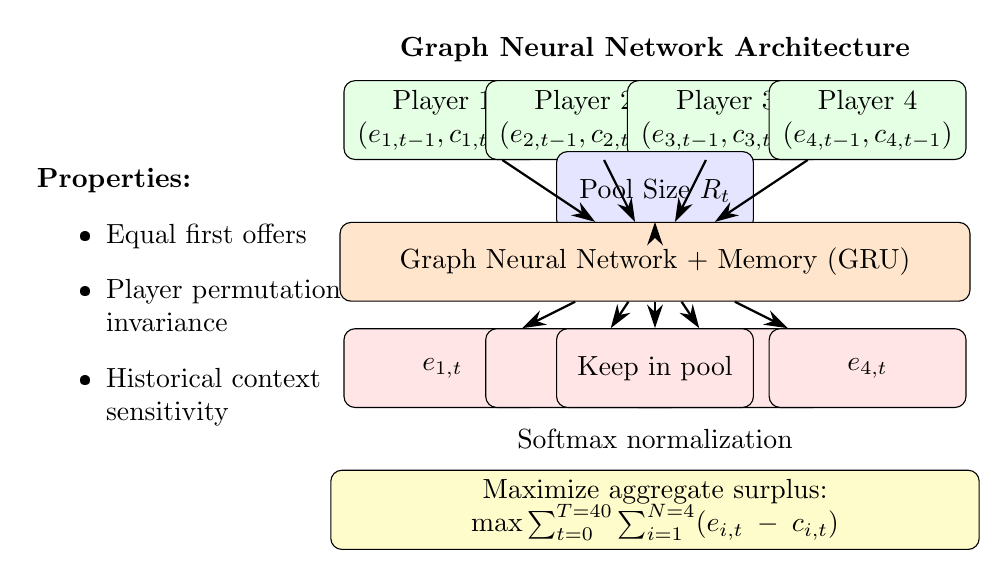
\begin{tikzpicture}[scale=0.9,
    block/.style={draw, rounded corners, minimum width=2.5cm, minimum height=1cm, align=center},
    arrow/.style={-{Stealth[length=3mm, width=2mm]}, thick}
]
    % Graph Neural Network
    \node[align=center] at (0,3) {\textbf{Graph Neural Network Architecture}};
    
    % Input nodes
    \node[block, fill=green!10] (p1) at (-3,2) {Player 1\\$(e_{1,t-1}, c_{1,t-1})$};
    \node[block, fill=green!10] (p2) at (-1,2) {Player 2\\$(e_{2,t-1}, c_{2,t-1})$};
    \node[block, fill=green!10] (p3) at (1,2) {Player 3\\$(e_{3,t-1}, c_{3,t-1})$};
    \node[block, fill=green!10] (p4) at (3,2) {Player 4\\$(e_{4,t-1}, c_{4,t-1})$};
    
    % Pool info
    \node[block, fill=blue!10] (pool) at (0,1) {Pool Size $R_t$};
    
    % GNN 
    \node[block, fill=orange!20, minimum width=8cm] (gnn) at (0,0) {Graph Neural Network + Memory (GRU)};
    
    % Outputs
    \node[block, fill=red!10] (a1) at (-3,-1.5) {$e_{1,t}$};
    \node[block, fill=red!10] (a2) at (-1,-1.5) {$e_{2,t}$};
    \node[block, fill=red!10] (a3) at (1,-1.5) {$e_{3,t}$};
    \node[block, fill=red!10] (a4) at (3,-1.5) {$e_{4,t}$};
    \node[block, fill=red!10] (keep) at (0,-1.5) {Keep in pool};
    
    % Softmax
    \node at (0,-2.5) {Softmax normalization};
    
    % Objective function
    \node[align=center, draw, fill=yellow!20, rounded corners, text width=8cm] at (0,-3.5) {Maximize aggregate surplus: $\max \sum_{t=0}^{T=40}\sum_{i=1}^{N=4}(e_{i,t} - c_{i,t})$};
    
    % Connections
    \draw[arrow] (p1) -- (gnn);
    \draw[arrow] (p2) -- (gnn);
    \draw[arrow] (p3) -- (gnn);
    \draw[arrow] (p4) -- (gnn);
    \draw[arrow] (pool) -- (gnn);
    
    \draw[arrow] (gnn) -- (a1);
    \draw[arrow] (gnn) -- (a2);
    \draw[arrow] (gnn) -- (a3);
    \draw[arrow] (gnn) -- (a4);
    \draw[arrow] (gnn) -- (keep);
    
    % Properties
    \node[align=left, text width=4cm] at (-6.5,-0.5) {
        \textbf{Properties:}
        \begin{itemize}
            \item Equal first offers
            \item Player permutation invariance 
            \item Historical context sensitivity
        \end{itemize}
    };
\end{tikzpicture}
\end{center}
\end{frame}

\section{Results}

\begin{frame}{Baseline Mechanism Results}
\begin{center}
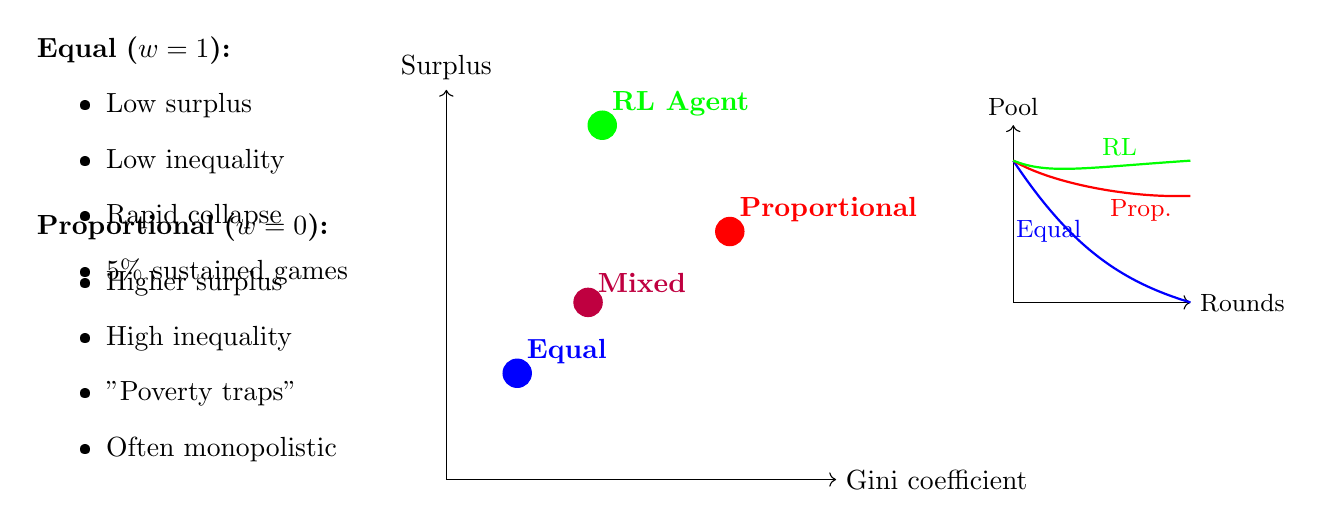
\begin{tikzpicture}[scale=0.9]
    % Create the coordinate system
    \draw[->] (0,0) -- (5.5,0) node[right] {Gini coefficient};
    \draw[->] (0,0) -- (0,5.5) node[above] {Surplus};
    
    % Data points
    \filldraw[blue] (1,1.5) circle (0.2) node[above right] {\textbf{Equal}};
    \filldraw[purple] (2,2.5) circle (0.2) node[above right] {\textbf{Mixed}};
    \filldraw[red] (4,3.5) circle (0.2) node[above right] {\textbf{Proportional}};
    \filldraw[green] (2.2,5) circle (0.2) node[above right] {\textbf{RL Agent}};
    
    % Annotations
    \node[align=left, text width=5cm] at (-3,4.5) {
        \textbf{Equal ($w = 1$):}
        \begin{itemize}
            \item Low surplus
            \item Low inequality
            \item Rapid collapse
            \item 5\% sustained games
        \end{itemize}
    };
    
    \node[align=left, text width=5cm] at (-3,2) {
        \textbf{Proportional ($w = 0$):}
        \begin{itemize}
            \item Higher surplus
            \item High inequality
            \item "Poverty traps"
            \item Often monopolistic
        \end{itemize}
    };
    
    % Example trajectories
    \begin{scope}[xshift=8cm, yshift=2.5cm]
        \draw[->] (0,0) -- (2.5,0) node[right, font=\small] {Rounds};
        \draw[->] (0,0) -- (0,2.5) node[above, font=\small] {Pool};
        
        \draw[blue, thick] (0,2) .. controls (0.8,0.8) and (1.5,0.3) .. (2.5,0);
        \draw[red, thick] (0,2) .. controls (0.5,1.7) and (1.5,1.5) .. (2.3,1.5) -- (2.5,1.5);
        \draw[green, thick] (0,2) .. controls (0.5,1.8) and (1,1.9) .. (2.5,2);
        
        \node[font=\small, blue] at (0.5,1) {Equal};
        \node[font=\small, red] at (1.8,1.3) {Prop.};
        \node[font=\small, green] at (1.5,2.2) {RL};
    \end{scope}
\end{tikzpicture}
\end{center}
\end{frame}

\begin{frame}{RL Agent Performance}
\begin{center}
\begin{tikzpicture}[scale=0.8]
    % Left panel - key metrics
    \node[align=left, text width=5cm] at (-3.5,1.5) {
        \textbf{RL Agent Results:}
        \begin{itemize}
            \item \textcolor{green!70!black}{150\% greater surplus}
            \item \textcolor{green!70!black}{Moderate inequality (Gini ≈ 0.2)}
            \item \textcolor{green!70!black}{65\% games sustained to end}
            \item \textcolor{green!70!black}{55\% with all four players}
        \end{itemize}
    };
    
    % Right panel - correlation visual
    \begin{scope}[xshift=3cm, yshift=1.5cm]
        \draw[->] (0,0) -- (4,0) node[right] {Gini};
        \draw[->] (0,0) -- (0,4) node[above] {Surplus};
        
        % Proportional baseline correlation
        \node at (2,3.5) {Proportional Baseline};
        \draw[red, thick, ->] (1,2) -- (3,3);
        \node[red, align=center, font=\small] at (2,1.3) {Higher surplus = \\Higher inequality\\$r = +0.69$};
        
        % RL correlation
        \node at (2,-0.5) {RL Agent (Sustained Games)};
        \draw[green, thick, ->] (1,-2) -- (3,-3);
        \node[green, align=center, font=\small] at (2,-3.7) {Higher surplus = \\Lower inequality\\$r = -0.5$};
    \end{scope}
    
    \node[align=center, draw, fill=yellow!20, rounded corners] at (-3.5,-2) {
        \textbf{Key Achievement:}\\RL created positive relationship between prosperity and equality
    };
\end{tikzpicture}
\end{center}
\end{frame}

\begin{frame}{What Made the RL Agent Successful?}
\begin{center}
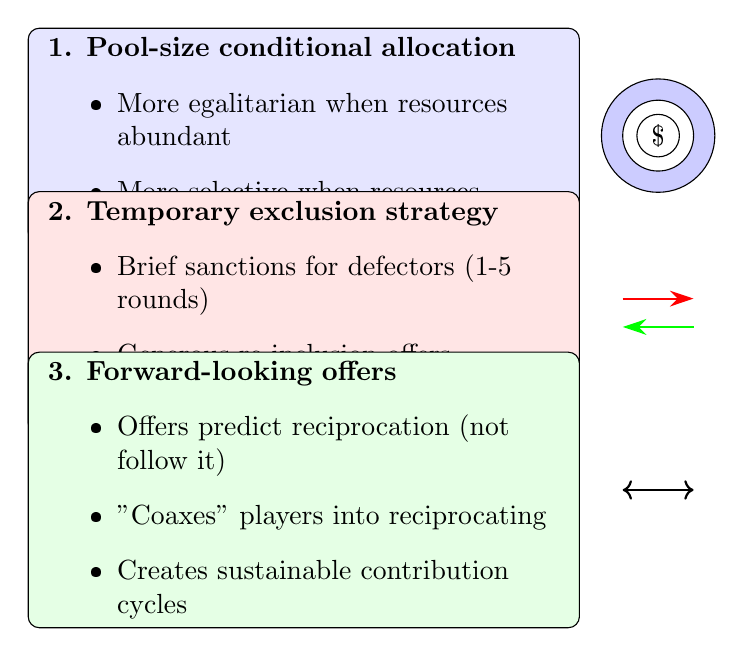
\begin{tikzpicture}[scale=0.9,
    strat/.style={draw, rounded corners, minimum width=7cm, minimum height=1.5cm, align=left, text width=6.5cm}]
    
    % Strategy 1
    \node[strat, fill=blue!10] (s1) at (0,2.5) {
        \textbf{1. Pool-size conditional allocation}
        \begin{itemize}
            \item More egalitarian when resources abundant
            \item More selective when resources scarce
        \end{itemize}
    };
    
    % Strategy 2
    \node[strat, fill=red!10] (s2) at (0,0) {
        \textbf{2. Temporary exclusion strategy}
        \begin{itemize}
            \item Brief sanctions for defectors (1-5 rounds)
            \item Generous re-inclusion offers
            \item Similar to "generous tit-for-tat"
        \end{itemize}
    };
    
    % Strategy 3
    \node[strat, fill=green!10] (s3) at (0,-2.5) {
        \textbf{3. Forward-looking offers}
        \begin{itemize}
            \item Offers predict reciprocation (not follow it)
            \item "Coaxes" players into reciprocating
            \item Creates sustainable contribution cycles
        \end{itemize}
    };
    
    % Images/icons for strategies
    \begin{scope}[xshift=5cm, yshift=2.5cm]
        \draw[fill=blue!20] (0,0) circle (0.8);
        \draw[fill=white] (0,0) circle (0.5);
        \draw (0,0) circle (0.3);
        \node at (0,0) {\$};
    \end{scope}
    
    \begin{scope}[xshift=5cm, yshift=0]
        \draw[-{Stealth[length=3mm, width=2mm]}, thick, red] (-0.5,0.2) -- (0.5,0.2);
        \draw[-{Stealth[length=3mm, width=2mm]}, thick, green] (0.5,-0.2) -- (-0.5,-0.2);
    \end{scope}
    
    \begin{scope}[xshift=5cm, yshift=-2.5cm]
        \draw[<->, thick] (-0.5,0) -- (0.5,0);
    \end{scope}
\end{tikzpicture}
\end{center}
\end{frame}

\begin{frame}{Creating an Explainable Mechanism}
\begin{center}
\begin{tikzpicture}[scale=0.9]
    % RL agent neural network (complex)
    \node[align=center] at (-3,3) {RL Agent Mechanism\\(Complex Neural Network)};
    \begin{scope}[xshift=-3cm, yshift=1.5cm]
        \node[draw, rounded corners, fill=blue!10, minimum width=3cm, minimum height=2cm] {
            \begin{tikzpicture}[scale=0.6]
                \foreach \x in {0,...,3} {
                    \foreach \y in {0,...,2} {
                        \node[draw, circle, fill=blue!20, minimum size=0.6cm] at (\x,\y) {};
                    }
                }
                \foreach \x in {0,...,3} {
                    \foreach \y in {0,...,2} {
                        \foreach \xx in {0,...,3} {
                            \foreach \yy in {0,...,2} {
                                \draw[-, opacity=0.1] (\x,\y) -- (\xx,\yy);
                            }
                        }
                    }
                }
            \end{tikzpicture}
        };
    \end{scope}
    
    % Arrow
    \draw[-{Stealth[length=5mm, width=3mm]}, thick, primcolor] (-1,1.5) -- (1,1.5);
    
    % Explainable mechanism
    \node[align=center] at (3,3) {Interpolating Baseline\\(Simple, Explainable)};
    \begin{scope}[xshift=3cm, yshift=1.5cm]
        \node[draw, rounded corners, fill=yellow!10, minimum width=3cm, minimum height=2cm] {
            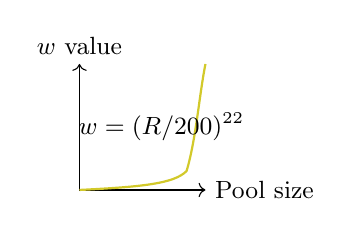
\begin{tikzpicture}[scale=0.8]
                \draw[->] (0,0) -- (2,0) node[right, font=\small] {Pool size};
                \draw[->] (0,0) -- (0,2) node[above, font=\small] {$w$ value};
                \draw[yellow!80!black, thick] (0,0) .. controls (1,0.05) and (1.5,0.1) .. (1.7,0.3) .. controls (1.85,0.8) and (1.9,1.5) .. (2,2);
                \node[font=\small] at (1.3,1) {$w = (R/200)^{22}$};
            \end{tikzpicture}
        };
    \end{scope}
    
    % Formula
    \node[align=center, fill=yellow!10, draw, rounded corners] at (0,-0.5) {$e_{i,t} = w \cdot \frac{R_t}{p} + (1-w) \cdot R_t \cdot \frac{c_{i,t-1}}{\sum_j c_{j,t-1}}$\\where $w = (R/200)^{22}$};
    
    % Results comparison
    \node[align=left, text width=6cm] at (-4.5,-2.5) {
        \textbf{Comparable performance:}
        \begin{itemize}
            \item Similar surplus
            \item Even lower Gini coefficient
            \item Higher player satisfaction
        \end{itemize}
    };
    
    % Human preferences
    \node[align=left, text width=6cm] at (4.5,-2.5) {
        \textbf{Human preferences:}
        \begin{itemize}
            \item Rated as fairer
            \item More understandable
            \item Preferred for future games
        \end{itemize}
    };
\end{tikzpicture}
\end{center}
\end{frame}

\begin{frame}{Longitudinal Study Results}
\begin{center}
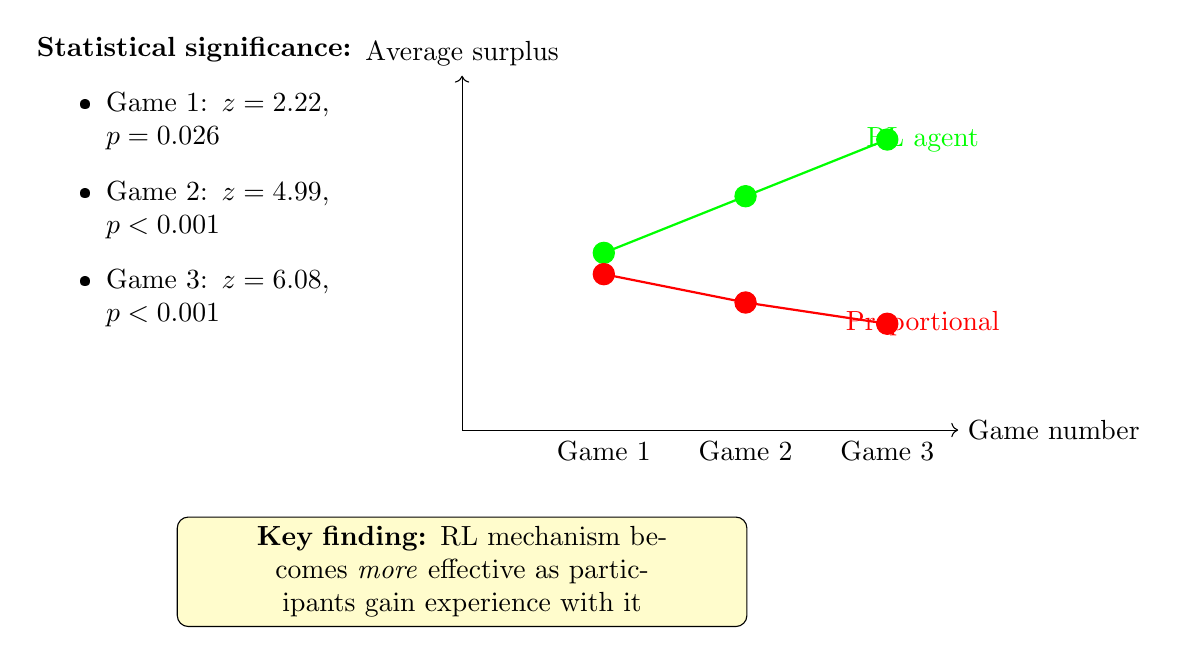
\begin{tikzpicture}[scale=0.9]
    % Coordinate system
    \draw[->] (0,0) -- (7,0) node[right] {Game number};
    \draw[->] (0,0) -- (0,5) node[above] {Average surplus};
    
    % X axis labels
    \node at (2,-0.3) {Game 1};
    \node at (4,-0.3) {Game 2};
    \node at (6,-0.3) {Game 3};
    
    % RL data points
    \filldraw[green] (2,2.5) circle (0.15);
    \filldraw[green] (4,3.3) circle (0.15);
    \filldraw[green] (6,4.1) circle (0.15);
    
    % Proportional data points
    \filldraw[red] (2,2.2) circle (0.15);
    \filldraw[red] (4,1.8) circle (0.15);
    \filldraw[red] (6,1.5) circle (0.15);
    
    % Connect points
    \draw[green, thick] (2,2.5) -- (4,3.3) -- (6,4.1);
    \draw[red, thick] (2,2.2) -- (4,1.8) -- (6,1.5);
    
    % Labels
    \node[green] at (6.5,4.1) {RL agent};
    \node[red] at (6.5,1.5) {Proportional};
    
    % Statistics
    \node[align=left, text width=4.5cm] at (-3.5,3.5) {
        \textbf{Statistical significance:}
        \begin{itemize}
            \item Game 1: $z = 2.22$, $p = 0.026$
            \item Game 2: $z = 4.99$, $p < 0.001$
            \item Game 3: $z = 6.08$, $p < 0.001$
        \end{itemize}
    };
    
    % Key finding
    \node[align=center, fill=yellow!20, draw, rounded corners, text width=7cm] at (0,-2) {
        \textbf{Key finding:} RL mechanism becomes \textit{more} effective as participants gain experience with it
    };
\end{tikzpicture}
\end{center}
\end{frame}

\section{Evaluation}

\begin{frame}{Key Strengths}
\begin{center}
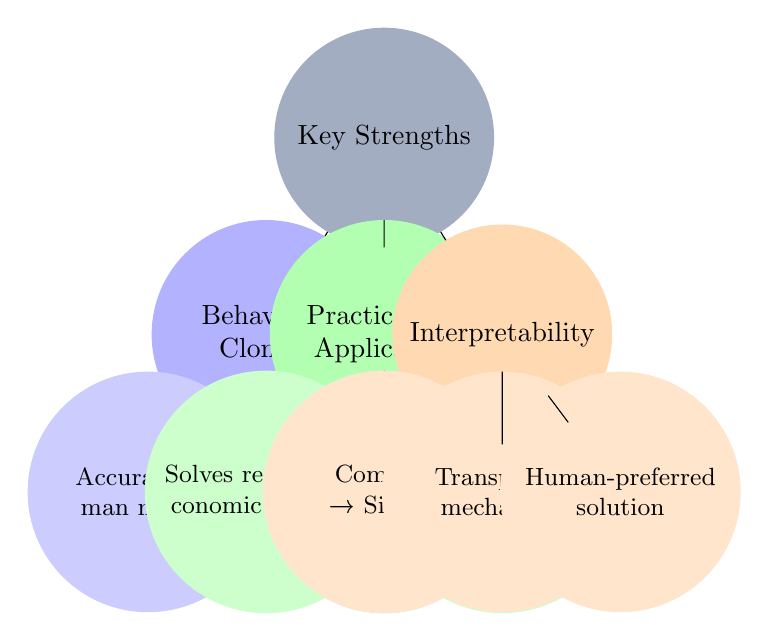
\begin{tikzpicture}[
    mind/.style={concept, concept color=primcolor!40, minimum size=2cm, text width=2.5cm, align=center},
    submind/.style={concept, concept color=primcolor!20, minimum size=1.5cm, text width=2.7cm, align=center, font=\small}
]
    \tikzset{level 1/.style={level distance=2.5cm}}
    \tikzset{level 2/.style={level distance=2cm}}

    \node[mind] {Key Strengths}
    child { node[mind, concept color=blue!30] {Behavioral Cloning}
        child { node[submind, concept color=blue!20] {Accurate human models} }
        child { node[submind, concept color=blue!20] {Rapid experimentation} }
        child { node[submind, concept color=blue!20] {Predictive accuracy} }
    }
    child { node[mind, concept color=green!30] {Practical RL Application}
        child { node[submind, concept color=green!20] {Solves real socioeconomic problem} }
        child { node[submind, concept color=green!20] {Discovers non-obvious strategies} }
        child { node[submind, concept color=green!20] {Informs policy design} }
    }
    child { node[mind, concept color=orange!30] {Interpretability}
        child { node[submind, concept color=orange!20] {Complex → Simple} }
        child { node[submind, concept color=orange!20] {Transparent mechanism} }
        child { node[submind, concept color=orange!20] {Human-preferred solution} }
    };
\end{tikzpicture}
\end{center}
\end{frame}

\begin{frame}{Limitations}
\begin{center}
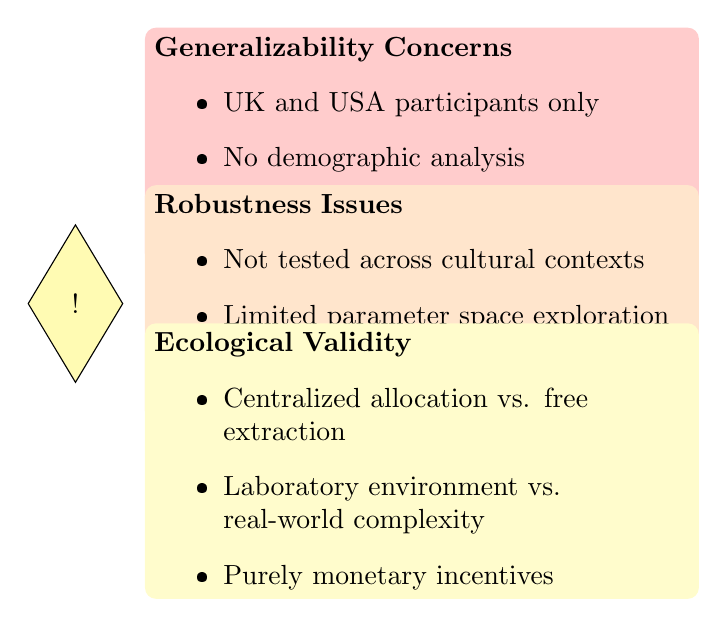
\begin{tikzpicture}[
    item/.style={rectangle, rounded corners, fill=#1!20, minimum width=7cm, minimum height=1.2cm, align=left, text width=6.8cm}
]
    % Generalizability concerns
    \node[item=red] (gen) at (0,2.5) {
        \textbf{Generalizability Concerns}
        \begin{itemize}
            \item UK and USA participants only
            \item No demographic analysis
            \item Simplified game vs. complex real-world scenarios
        \end{itemize}
    };
    
    % Robustness issues
    \node[item=orange] (rob) at (0,0.5) {
        \textbf{Robustness Issues}
        \begin{itemize}
            \item Not tested across cultural contexts
            \item Limited parameter space exploration
            \item Potential sensitivity to initial conditions
        \end{itemize}
    };
    
    % Ecological validity
    \node[item=yellow] (eco) at (0,-1.5) {
        \textbf{Ecological Validity}
        \begin{itemize}
            \item Centralized allocation vs. free extraction
            \item Laboratory environment vs. real-world complexity
            \item Purely monetary incentives
        \end{itemize}
    };
    
    % Warning sign
    \begin{scope}[xshift=-5cm, yshift=0.5cm]
        \draw[fill=yellow!30] (0,0) -- (0.6,1) -- (1.2,0) -- (0.6,-1) -- cycle;
        \node at (0.6,0) {!};
    \end{scope}
\end{tikzpicture}
\end{center}
\end{frame}

\section{Discussion}

\begin{frame}{Discussion}
\begin{center}
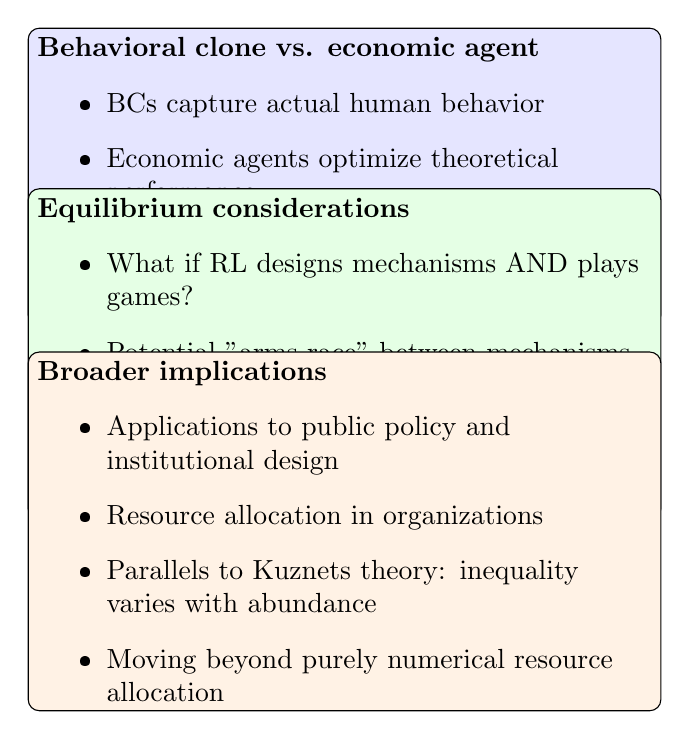
\begin{tikzpicture}[scale=0.9,
    block/.style={draw, rounded corners, minimum width=8cm, minimum height=2cm, align=left, text width=7.8cm}
]
    % Behavioral clone vs economic agent
    \node[block, fill=blue!10] (bc) at (0,2) {
        \textbf{Behavioral clone vs. economic agent}
        \begin{itemize}
            \item BCs capture actual human behavior
            \item Economic agents optimize theoretical performance
            \item Trade-off: Reality vs. optimality
            \item BCs may handle policy shifts more naturally
        \end{itemize}
    };
    
    % Equilibrium considerations
    \node[block, fill=green!10] (eq) at (0,-0.5) {
        \textbf{Equilibrium considerations}
        \begin{itemize}
            \item What if RL designs mechanisms AND plays games?
            \item Potential "arms race" between mechanisms and players
            \item Long-term stability of discovered solutions
            \item Evolutionary dynamics between strategies
        \end{itemize}
    };
    
    % Broader implications
    \node[block, fill=orange!10] (br) at (0,-3) {
        \textbf{Broader implications}
        \begin{itemize}
            \item Applications to public policy and institutional design
            \item Resource allocation in organizations
            \item Parallels to Kuznets theory: inequality varies with abundance
            \item Moving beyond purely numerical resource allocation
        \end{itemize}
    };
\end{tikzpicture}
\end{center}
\end{frame}

\begin{frame}{Future Directions}
\begin{center}
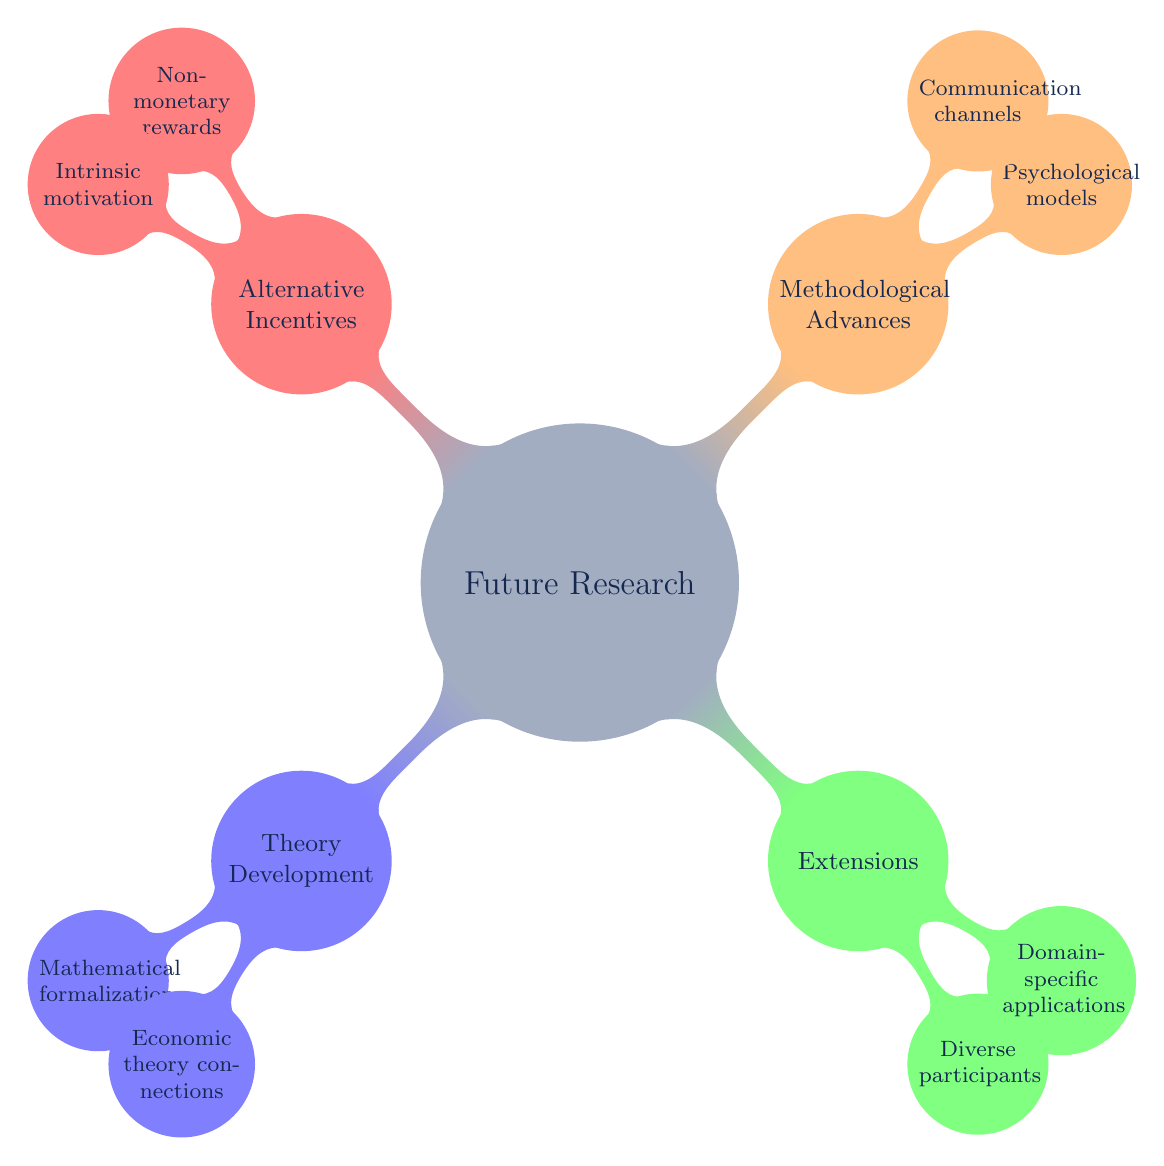
\begin{tikzpicture}[mindmap, concept color=primcolor!40, text=primcolor!80!black]
    \node[concept] {Future Research}
      child[concept color=blue!50, grow=225] { node[concept] {Theory Development} 
        child { node[concept] {Mathematical\\formalization} }
        child { node[concept] {Economic\\theory connections} }
      }
      child[concept color=green!50, grow=315] { node[concept] {Extensions} 
        child { node[concept] {Diverse\\participants} }
        child { node[concept] {Domain-specific\\applications} }
      }
      child[concept color=orange!50, grow=45] { node[concept] {Methodological\\Advances} 
        child { node[concept] {Psychological\\models} }
        child { node[concept] {Communication\\channels} }
      }
      child[concept color=red!50, grow=135] { node[concept] {Alternative\\Incentives} 
        child { node[concept] {Non-monetary\\rewards} }
        child { node[concept] {Intrinsic\\motivation} }
      };
\end{tikzpicture}
\end{center}
\end{frame}

\begin{frame}{Conclusion}
\begin{center}
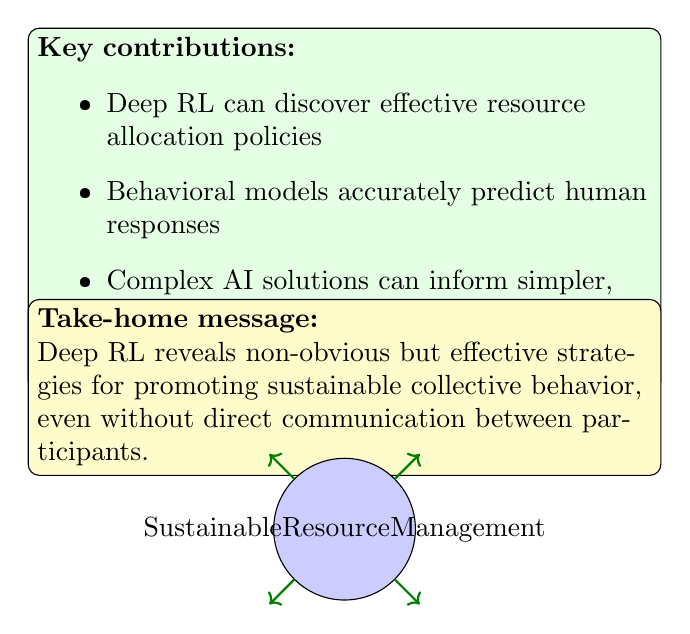
\begin{tikzpicture}[scale=0.9,
    box/.style={draw, rounded corners, minimum width=8cm, text width=7.8cm, align=left}
]
    % Main contributions
    \node[box, fill=green!10, minimum height=2.5cm] (contrib) at (0,2) {
        \textbf{Key contributions:}
        \begin{itemize}
            \item Deep RL can discover effective resource allocation policies
            \item Behavioral models accurately predict human responses
            \item Complex AI solutions can inform simpler, practical policies
            \item Balancing prosperity and equality is possible
        \end{itemize}
    };
    
    % Takeaway message
    \node[box, fill=yellow!20, minimum height=1.5cm] (takeaway) at (0,-0.5) {
        \textbf{Take-home message:}\\
        Deep RL reveals non-obvious but effective strategies for promoting sustainable collective behavior, even without direct communication between participants.
    };
    
    % Visual representation
    \begin{scope}[xshift=0cm, yshift=-2.5cm]
        \draw[fill=blue!20] (0,0) circle (1);
        \foreach \angle in {45, 135, 225, 315} {
            \draw[thick, green!50!black, ->] (\angle:1) -- (\angle:1.5);
        }
        \node at (0,0) {Sustainable\\Resource\\Management};
    \end{scope}
\end{tikzpicture}
\end{center}
\end{frame}

\begin{frame}{References}
\begin{itemize}
    \item Koster, R., Pîslar, M., Tacchetti, A., Balaguer, J., Liu, L., Elie, R., Hauser, O.P., Tuyls, K., Botvinick, M., \& Summerfield, C. (2025). Deep reinforcement learning can promote sustainable human behaviour in a common-pool resource problem. \textit{Nature Communications}, 16(2824).
    
    \item Koster, R., et al. (2022). Human-centred mechanism design with democratic AI. \textit{Nature Human Behaviour}, 6, 1398-1407.
    
    \item Ostrom, E. (1991). Governing the Commons: The Evolution of Institutions for Collective Action. Cambridge University Press.
    
    \item Fehr, E., \& Gächter, S. (2002). Altruistic punishment in humans. \textit{Nature}, 415, 137-140.
\end{itemize}
\end{frame}

\end{document}